

\section{Introduction}
Vision impairment is one of the health problems experienced by many people around the world. It is estimated that more than 2.2 billion people worldwide have vision impairment, and at least 1 billion of them have vision impairments that are actually preventable or have not been adequately treated. Some of the diseases that can cause vision loss or even blindness are cataracts, diabetic retinopathy, and glaucoma \cite{WHO2023Blindness}. About 15.2 million people experience blindness due to cataracts, or about 45\% of all global blindness cases. In addition, cataracts are also the second largest cause of moderate to severe visual impairment, experienced by around 78.8 million people \cite{GBD2024Cataract}. Meanwhile, diabetic retinopathy continues to increase as the number of people with diabetes mellitus increases, with around 20\%–35\% of diabetics estimated to have diabetic retinopathy \cite{Pan2025DR}. The number of cases is projected to reach 129.84 million by 2030 and 160.50 million by 2045 \cite{Pan2025DR}. Glaucoma, as the leading cause of irreversible blindness in the world, is estimated to affect around 76 million people in 2020 and is projected to increase to 111.8 million people by 2040, with Asia and Africa being the most affected regions \cite{Vania2024Glaucoma}. These epidemiological facts underscore the urgency of developing accurate, affordable, and scalable early detection systems, particularly in low- and middle-income countries that face limited access to ophthalmological personnel.
\begin{figure*}[t]
    \centering
    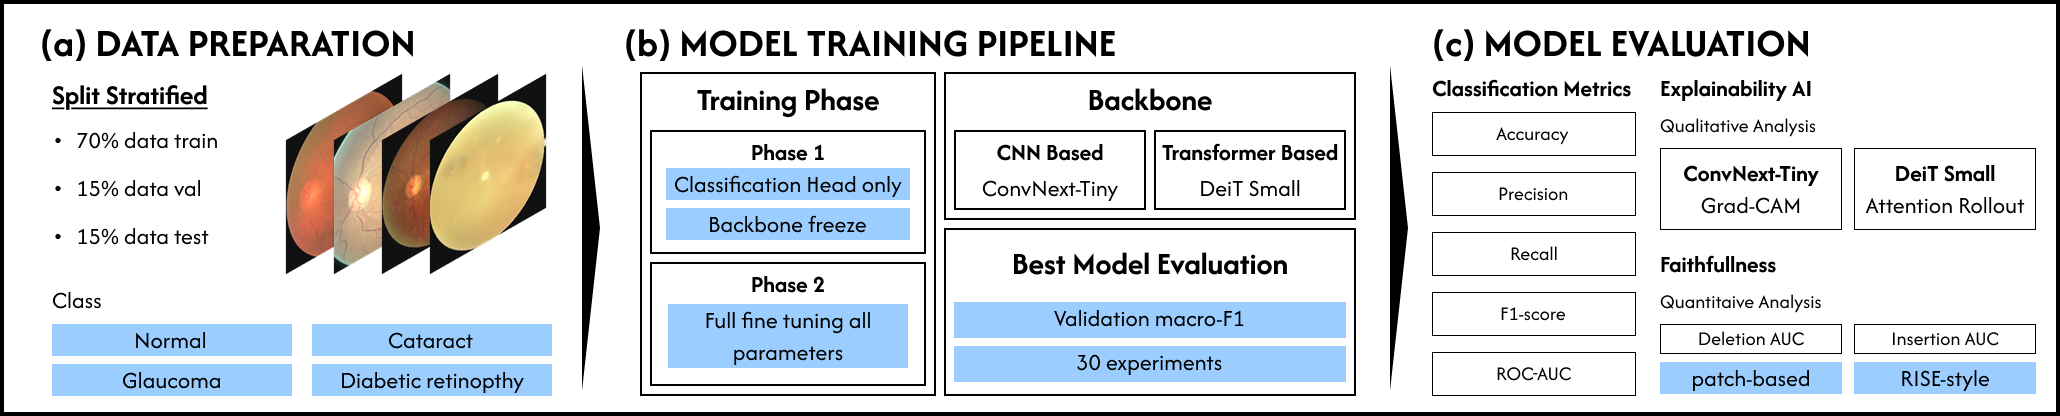
\includegraphics[width=\textwidth]{figures/methodology_version1}
    \caption{Overview of the research methodology.}
    \label{fig:methodology_overview}
\end{figure*}

To answer this need, a deep learning-based approach have been widely used in medical image analysis because it is able to extract features automatically from fundus images and other ophthalmological images without the need for manual feature extraction processes \cite{Elkholy2024OCT}. The development of deep learning architecture presents two main approaches, namely Convolutional Neural Network (CNNs) and Vision Transformer (ViTs). One of the latest CNN architectures is ConvNeXt, which was developed by adopting some of the design principles of the Vision Transformer so that it can improve accuracy while maintaining CNN efficiency \cite{Liu2022}. On the other hand, the Vision Transformer (ViT) uses a self-attention mechanism to learn the relationships between parts of the image. One of the developments is the Data-efficient Image Transformer (DeiT), which allows models to be trained effectively using smaller datasets with lower computational requirements through knowledge distillation techniques \cite{touvron2021trainingdataefficientimagetransformers}.

Although deep learning models have very high classification accuracy, they often suffer from a black-box limitation. This means that the model can provide accurate predictions, but the process behind its decision-making is not transparent and is difficult for humans to understand \cite{Gomez2022Saliency}. Therefore, Explainable Artificial Intelligence (XAI) technology is used to visualize the reasoning behind the model's predictions. For models that use CNN architecture such as ConvNeXt, the Grad-CAM method is typically used to create a heatmap that highlights the most important areas of the image. Meanwhile, in Transformer architectures such as DeiT, the method used is Attention Rollout or Gradient Attention Rollout. This method works by collecting the attention weights of each layer of the model to see which parts of the image the model is most focused on \cite{Cho2025GMAR}. The different internal mechanisms of these two models mean that the quality of the resulting visualizations is not directly comparable. The main problem is that current deep learning evaluations in the medical field mostly stop at accuracy comparison. To quantitatively measure how faithful these visualizations are, specific metrics are required. Deletion and insertion metrics that use Area Under Curve (AUC) values are often used as the standard of measurement. These metrics work by gradually hiding or showing parts of the image according to their importance, and then seeing how much the model's confidence level in its predictions changes \cite{Gomez2022Saliency}.  

Based on the problems that have been described, the focus of this research is formulated into two main analytical scopes. The first focus is on a comparative evaluation of the classification performance between the ConvNeXt and DeiT architectures on a dataset of four classes of eye diseases (cataracts, diabetic retinopathy, glaucoma, and normal) using accuracy, precision, recall, and F1-score metrics. The second focus is a comparative analysis of the quality of visual explanations, particularly at the level of faithfulness of heatmap representation, between the Grad-CAM method in the ConvNeXt model and the Attention Rollout in the DeiT model, which is quantitatively evaluated through deletion AUC and insertion AUC measurements.

To address these problems, this research presents two main contributions. Theoretically, this study enriches the academic literature related to the comparative interpretability between modern CNN (ConvNeXt) and Vision Transformer (DeiT) architectures that are specialized in the domain of ophthalmological medical imaging. previous research that rarely explored the comparison of models in depth based on the faithfulness parameters of XAI visualizations, instead of relying solely on accuracy metrics. Meanwhile, practically, this study provides an empirical evidence-based guideline for clinical practitioners and engineers in determining the combination of XAI architecture and methods that best suits the needs of operational systems. For example, the results of this research can be used as a direct reference in choosing the most recommended architecture when a diagnostic system requires a heatmap localization that is highly aligned with the model's decision-making basis.
